\documentclass[tikz,border=4pt]{standalone}
\usetikzlibrary{angles,quotes}
\begin{document}
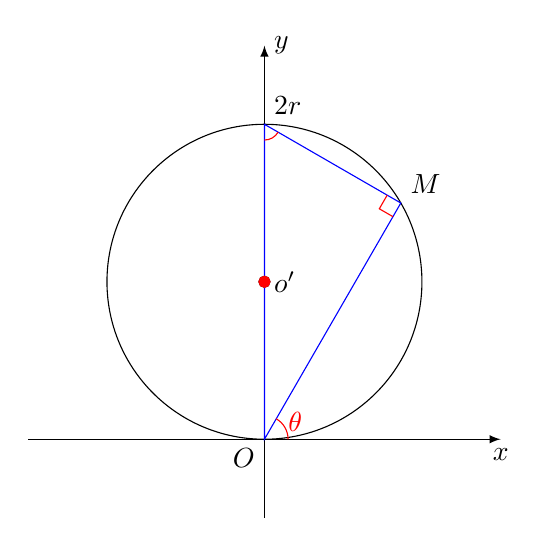
\begin{tikzpicture}[>=latex]
    \draw[->] (-3,0) -- (3,0) coordinate(x-axis) node[below] {$x$};
    \draw[->] (0,-1) -- (0,5) node[right]{$y$};
    \draw (0,2) circle[radius=2] circle[fill,radius=2pt] node[right] {$o'$};
    \coordinate[label=below left:$O$] (C);
    \coordinate[label=above right:$2r$] (A) at (0,4);
    \coordinate[label=above right:$M$] (B) at (1.732,3);
    \draw[blue] (A) -- (B) -- (C) --cycle;
    \filldraw[red] (0,2) circle[radius=2pt];
    \pic[red,draw,angle radius=2mm]{right angle=A--B--C};
    \pic[red,draw,angle radius=2mm]{angle=C--A--B};
    \pic["$\theta$",angle eccentricity=1.5,red,draw,angle radius=3mm]{angle=x-axis--C--B};
\end{tikzpicture}
\end{document}